% A pilot: two capped readouts fused. Input by main.tex; kept to one page. Its theory,
% derivation, setup in full and remaining results are in fusion_appendix.tex. Every measured
% value is a macro from numbers.tex, read from results/fusion_experiment.json by
% paper/make_numbers.py.
% =========================================================================================
\section{A pilot: two capped readouts fused}
\label{sec:fusion}

This section is a pilot, and what it does not show comes first. It uses one dataset,
N-MNIST. Its second input is a degraded copy from the same sensor, not a second modality: a
different test sample of the same class, read by the same network after each event is
removed with probability \fuRate. No fusion network is trained. There is no reference-frame % src: results/fusion_dropout_rate.json
transformation between the two inputs, and no closed loop: the fused decision is scored, not
acted on.

\paragraph{What it tests.}
A source known only by its accuracy $a$ is weighted by $\ln\big((C-1)a/(1-a)\big)$ in
decision-fusion theory~\citep{shapley1984optimizing,kuncheva2014weighted,li2014error}, the % [LIT] shapley1984optimizing, Theorem II; kuncheva2014weighted, Eq. (15); li2014error, Corollary 9
minimum logit width of Equation~\eqref{eq:tmin}, and calibrating each source before combining is
the standard remedy for confidences that cannot be trusted~\citep{brummer2007fusion,kumar2022calibrated}. % [LIT] brummer2007fusion, Section IV; kumar2022calibrated, Proposition 4.1
A count readout is \emph{saturated} when its winner fires at all $T$ steps and no other class
fires; its output is then the ceiling of Equation~\eqref{eq:ceiling}, one vector up to which
class wins. Where both inputs saturate, an event $S$, the product
rule~\citep{kittler1998combining} cannot weight one input above the other and becomes an % [LIT] kittler1998combining, Section 2.1
unweighted vote. Against a rule that sides with input A on every disagreement in $S$ it loses
\begin{equation}
\tfrac12\,P(S)\,\big(a_{A,S}-a_{B,S}\big)
\label{eq:fusioncost}
\end{equation}
in accuracy, $a_{k,S}$ being input $k$'s accuracy on $S$, and a scale with
$s_kT=\ln\big((C-1)a_k/(1-a_k)\big)$ on each input's counts restores the weighting. This is a
corollary of known theory, not a new result; Appendix~\ref{app:fusion} derives it.

\paragraph{Setup and result.}
R0 is the product rule on the raw softmax outputs, R1 the product rule after temperature scaling
each input, and $\delta=\operatorname{acc}(\mathrm{R1})-\operatorname{acc}(\mathrm{R0})$, with 95\%
bootstrap intervals over \fuPairings{} pairings of the \nmSplitTest{} test samples in three seeds % src: results/fusion_experiment.json pairings; results/nmnist_T2_seed0_split.npz
(Appendix~\ref{app:fusionsetup}). At $T=2$ both inputs saturate on \fuTwoPSMin{} to % src: results/fusion_experiment.json p_s
\fuTwoPSMax{} of pairs, and calibrating first raises fused accuracy from \fuCountTwoRZero{} to % src: results/fusion_experiment.json acc_r0, acc_r1
\fuCountTwoROne: \fuTwoErrCut\% of the fused errors, but only \fuTwoDeltaPoints{} points. Every % src: results/fusion_experiment.json acc_r0, acc_r1, delta
seed's interval on $\delta$ excludes zero, and prediction 12 \verdictTwelve. % src: results/fusion_experiment.json predictions.12
Equation~\eqref{eq:fusioncost} lies inside the interval of the part of $\delta$ from $S$ in
\fuThirteenWithin{} of 3 seeds, and prediction 13 \verdictThirteen. From $T=4$ every interval % src: results/fusion_experiment.json predictions.13
includes zero (Figure~\ref{fig:fusion}), because two saturated inputs there almost never
disagree. Prediction 14 is \verdictFourteen, since its means at $T=6$ and $T=10$ are equal where % src: results/fusion_experiment.json predictions.14
it asked for a strict fall, and prediction 15 is \verdictFifteen, since \fuAccumExcl{} of % src: results/fusion_experiment.json predictions.15
\fuAccumRuns{} accumulator runs excludes zero, against calibration
(Appendix~\ref{app:fusionresults}).

\paragraph{Reliability from spikes, elsewhere.}
Grillo et al.\ weight a sensory signal delayed by 100\,ms against a cerebellar prediction in a
spiking state estimator in NEST, by reliabilities computed from the variability of spike counts
within each input population, tested on simulated inputs as an isolated block with each
population's variability set by the authors~\citep{grillo2022bayesian}. Here reliability is read % [LIT] grillo2022bayesian, Sections 2.1, 2.2 and 4
from a readout's confidence, which the cap limits.

\begin{figure}[t]
\begin{minipage}[b]{0.5\linewidth}
\centering
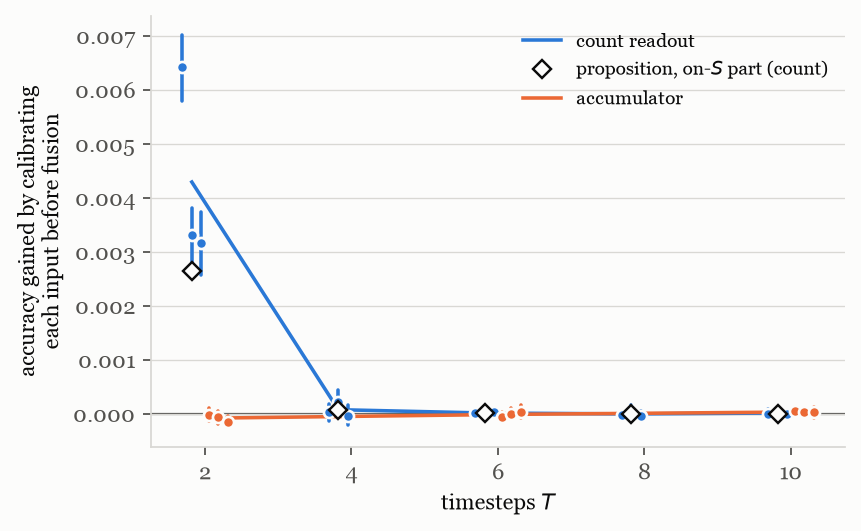
\includegraphics[width=\linewidth]{figures/fig9-fusion.png} % figures/fig9-fusion.png, drawn by spikecalib/figures.py from results/fusion_experiment.json
\caption{The pilot: $\delta$, the accuracy gained by calibrating each input before the product
rule, against $T$ on N-MNIST. Points are seeds with 95\% bootstrap intervals; open diamonds are
Equation~\eqref{eq:fusioncost}.} % src: results/fusion_experiment.json
\label{fig:fusion}
\end{minipage}\hfill
\begin{minipage}[b]{0.46\linewidth}
\centering
\small
\begin{tabular}{lrr}
\toprule
$T=2$ & count & accum. \\
\midrule
input A alone        & \fuCountTwoAccA    & \fuAccumTwoAccA \\ % src: results/fusion_experiment.json accuracy_a
input B alone        & \fuCountTwoAccB    & \fuAccumTwoAccB \\ % src: results/fusion_experiment.json accuracy_b
R0, raw product      & \fuCountTwoRZero   & \fuAccumTwoRZero \\ % src: results/fusion_experiment.json acc_r0
R1, calibrated first & \fuCountTwoROne    & \fuAccumTwoROne \\ % src: results/fusion_experiment.json acc_r1
$P(S)$               & \fuCountTwoPS      & -- \\ % src: results/fusion_experiment.json p_s
$\delta$             & \fuCountTwoDelta   & \fuAccumTwoDelta \\ % src: results/fusion_experiment.json delta
$\delta$ on $S$      & \fuCountTwoDeltaOnS & -- \\ % src: results/fusion_experiment.json delta_on_s
Eq.~\eqref{eq:fusioncost} & \fuCountTwoPredicted & -- \\ % src: results/fusion_experiment.json predicted_on_s
\bottomrule
\end{tabular}
\captionof{table}{The pilot at $T=2$, mean of three seeds and \fuPairings{} pairings. An % src: results/fusion_experiment.json pairings
accumulator has no counts, so nothing saturates. Every $T$ and the vote R2: Table~\ref{tab:fusionhigh}.}
\label{tab:fusion}
\end{minipage}
\end{figure}
